%TEX program = xelatex
\documentclass[12pt]{amsart}
\usepackage{amssymb}
\usepackage{amsmath}
\usepackage{mathrsfs}
\usepackage{mathbbol}
\usepackage{amsfonts}
\usepackage{amssymb,amsmath}
\usepackage{graphicx}
\graphicspath{{./images/}}
% \usepackage[pagewise]{lineno}\linenumbers
\oddsidemargin=-.0cm
\evensidemargin=-.0cm
\textwidth=16cm
\textheight=22cm
\topmargin=0cm
%%%%%%%%%%%%%%%%%%%%%%%%%%%%%%%%%%%%%%%%%%%%
% DEFS
\def\C {{\mathcal C}}

\def\R {\mathbb{R}}


\def\d{{\,\rm d}}

\def\i{{\rm i}}

%%%%%%%%%%%%%%%%%%%%%%%%%%%%%%%%%%%%%%%%%%%%

%%%%%%%%%%%%%%%%%%%%%%%%%%%%%%%%%%%%%%%%%%%%
\newtheorem{proposition}{Proposition}[section]
\newtheorem{theorem}[proposition]{Theorem}
\newtheorem{corollary}[proposition]{Corollary}
\newtheorem{lemma}[proposition]{Lemma}
\theoremstyle{definition}
\newtheorem{definition}[proposition]{Definition}
\newtheorem{example}[proposition]{Example}
\newtheorem{remark}[proposition]{Remark}
\numberwithin{equation}{section}
%%%%%%%%%%%%%%%%%%%%%%%%%%%%%%%%%%%%%%%%%%%%
% BIBLIOGRAPHY
\def \au {\rm}
\def \ti {\it}
\def \jou {\rm}
\def \bk {\it}
\def \no#1#2#3 {{\bf #1} (#3), #2.}
%\no{Vol}{Pag}{Year}
\def \eds#1#2#3 {#1, #2, #3.}
%\eds{Pub}{City}{Year}
%%%%%%%%%%%%%%%%%%%%%%%%%%%%%%%%%%%%%%%%%%%%%%%%%

\renewcommand\baselinestretch{1.3}

%%%%%%%%%%%%%%%%%%%%%%%%%%%%%%%%%%%%%%%%%%%%%%%%%
\title[Observability inequality ]
{ \bf
 Observability inequality at two time points for KdV equations from measurable sets}

\author[ ]
{    }


%\address{Ming Wang
%\newline\indent
%School of Mathematics and Physics, China University of Geosciences
%\newline\indent
%Wuhan, 430074,  China
%}
%\email{mwang@cug.edu.cn}


 

\subjclass[2010]{35Q55, 39A12}
\keywords{KdV equation,   unique continuation}

%%%%%%%%%%%%%%%%%%%%%%%%%%%%%%%%%%%%%%%%%%%%%%%%%



%%%%%%%%%%%%%%%%%%%%%%%%%%%%%%%%%%%%%%%%%%%%%%%%%
\begin{document}



%\begin{abstract}


%\keywords{KdV equation \and Global attractor \and Fractal dimension \and Bourgain space }
% \PACS{PACS code1 \and PACS code2 \and more}
%\subclass{35Q53  \and  35B41}
%\end{abstract}

\maketitle
\tableofcontents
%%%%%%%%%%%%%%%%%%%%%%%%%%%%%%%%%%%%%%%%%%%%%%%%%
\section{Introduction}
Let $\Omega \subset \R^{n}$ be an open domain.
Consider the following evolution equation 
\begin{equation}
    \partial_t u=Fu,\quad u(0,x)=u_0\in L^2(\Omega),\label{gen}
\end{equation}
where $F$ is a linear operator.
Sometimes we want to get the global information of the solution $u(t,x)$ of (\ref{gen}) at time $t$ out of a small region $\omega\subset \Omega$. For example, we may establish some inequalities such as 
\begin{equation}
    \int_{\Omega}|u(T,x)|^2\d x\le C(T,\Omega)\int_0^T\int_\omega |u(t,x)|^2\d x\d t,\label{genobs}
\end{equation}  
where $\omega\subset \Omega$ and $C(T,\Omega)$ is a constant depending on $T$ and $\Omega$.
An inequality like (\ref{genobs}) is called an observability inequality of (\ref{gen}).


Roughly speaking, Uncertainty Principle says that it is impossible for a nonzero function and its Fourier transform to have compact supports simultaneously. More precisely, we can illustrate this property by the following inequality:
\begin{equation}
    \int_{\R^n}|f(x)|^2\d x\le Ce^{Cr_1r_2}\left(\int_{|x|\ge r_1}|f|^2\d x+\int_{|x|\ge r_2}|\widehat{f}(\xi)|^2\d\xi\right).\label{un}
\end{equation}   
Here $C=C(n)$ is a constant and the inequality holds for all $r_1,r_2>0$ and all $f\in L^2(\R^n)$. This was proved by the Logvinenko-Sereda theorem in \cite{Log,Korv,Rouss,WWZZ} and was shown to directly follow from a Nazarov type uncertainty principle in \cite{Naza}.

Recently, G. Wang, M. Wang, Y. Zhang \cite{WWZ} found the connection between (\ref{un}) and the observability inequality for the free Schr\"{o}dinger equation
\begin{equation}
    i\partial_t u-\Delta u=0,\quad u(0,x)=u_0(x)\in L^2(\R^n).\label{sch}
\end{equation}
In fact, it was proved in \cite{WWZ} that (\ref{un}) is equivalent to the following: There exists a constant $C=C(n)>0$ such that for all $t>0$, all $r_1,r_2>0$ and all $u(t,x)$ solving   (\ref{sch}), 
\begin{equation}
    \int_{\R^n}|u_0(x)|^2\d x \le C e^{\frac{Cr_1r_2}{t}}\left(\int_{|x|\ge r_1} |u_0(x)|^2\d x+\int _{|x|\ge r_2}|u(t,x)|^2\d x\right).\label{sch-obs}
\end{equation}
This is an observability inequality of (\ref{sch}).

Here we are interested in the linear Korteweg-de Vries (KdV) equation
\begin{equation}
u_t+u_{xxx}=0, \quad u(0,x)=u_0(x)\in L^2(\R).\label{kdv}
\end{equation}
Our aim is to establish the similar observability inequality at two time points as (\ref{sch-obs}) for (\ref{kdv}). The newest result about this is accomplished by Z. Li and M. Wang in \cite{LW}: There exists a constant $C>0$ so that for all $r_1,r_2,t>0$ and all $u(t,x)\in C([0,\infty);L^2(\R))$ solving (\ref{kdv}),
\begin{equation}
    \int_{\R}|u_0(x)|^2\d x\le Ce^{Ct^{-\frac{4}{3}}\left(r_1^4+r_2^4\right)}\left(\int_{|x|\ge r_1}|u_0(x)|^2\d x+\int _{|x|\ge r_2}|u(t,x)|^2\d x\right).\label{lw}
\end{equation}
We will prove the following theorem 
\begin{theorem}\label{thm-1}
    Let $A,B$ be two  measurable sets in $\R$ with finite measure. Then for every $t>0$, there exists $C=C(t,|A|,|B|)>0$ so that when $u(t,x)$ solves the KdV equation,
    \begin{equation}
    \int_\R |u_0|^2\d x \leq C\left( \int_{A^c}|u_0|^2\d x + \int_{B^c}|u(t,x)|^2\d x \right).\label{kdv-obs}
    \end{equation}
    \end{theorem}
There is a major difference between  the result of Z. Li and M. Wang in \cite{LW} and Theorem \ref{thm-1}:
The inequality (\ref{lw}) gives an exact relation between the constant and $t,r_1,r_2$. The inequality (\ref{kdv-obs}) fails to give such a relation, but removes the bounded condtion of two sets $A$ and $B$.


Theorem \ref{thm-1} requires two sets $A$ and $B$ have finite measure. This limitation can be replaced by a more general condition (in which one of the sets may have infinite measure) in the case of Schr\"{o}dinger equations. We will find some type of  $A$ and $B$ with infinite measure and the inequality (\ref{kdv-obs}) still holds.

\begin{definition}
    We say the set $A$ has $|x|^{-\alpha}$ density if $\alpha>0$ and 
    $$
    \varlimsup_{x\to \infty}|A\bigcap[x,x+1]|\lesssim |x|^{-\alpha}.
    $$
\end{definition}
\begin{remark}
    It is equivalent to say that, there exists $L>0$ so that
    $$
        |A\bigcap[x,x+1]|\lesssim |x|^{-\alpha}, \quad \forall |x|\geq L.
    $$
\end{remark}
\begin{theorem}\label{thm-2}
    Let  $A$ and $B$ be measurable sets with density  $\alpha\in (\frac{5}{6},1)$, $A,B\subset (c,\infty)$ or $A,B\subset (-\infty,c)$  for some $c$. Then for every $t>0$, there exists $C=C(t,A,B)>0$ so that when $u(t,x)$  solves the KdV equation, (\ref{kdv-obs}) holds.     
\end{theorem}
\section{Projection operators}
\begin{definition}
    Suppose that $(\mathcal{H},\|\cdot\|)$ is a Hilbert space, $\{e_i\lvert i\in I\}$ is an orthonormal basis of $\mathcal{H}$. Then for any linear operator $T$ on $\mathcal{H}$ define 
    $$
        \| T\|^2_{\mathrm{HS}}\equiv \sum_{i\in I}\|Te_i\|^2.
    $$       
$\|T\|_{\mathrm{HS}}$ is called the Hilbert-Schmidt norm of $T$. Moreover, the bounded operator $T$ is a Hilbert-Schmidt operator if $\|T\|_{\mathrm{HS}}$ is finite.    
\end{definition}
\begin{lemma}\label{lma-1} 
    All Hilbert-Schmidt operators are compact.
\end{lemma}

\begin{proposition}\label{prop-2}
    Let $(\mathcal{H},\|\cdot\|)$ be an infinite-dimensional complex Hilbert space. Let $E$, $F$ be two orthogonal projections acting in $\mathcal{H}$ and $S:\mathcal{H}\to \mathcal{H}$ be an invertible operator. Define $E^{\perp}\equiv I-E$, $F^{\perp}\equiv I-F$ and $T=ESF$ . If $\|S^{-1}\|\|T\|<1$ , then there exists a constant $C>0$ sucht that for any $f\in \mathcal{H}$  
    \begin{equation}
        \|f\|\le C\left(\|E^{\perp}Sf\|+\|F^{\perp}f\|\right),\label{gen-1}
    \end{equation}      
    or equivalently a constant $C'>0$ such that for any $f\in \mathcal{H}$
    \begin{equation}
        \|f\|^2\le C'\left(\|E^{\perp}Sf\|^2+\|F^{\perp}f\|^2\right).\label{gen-2}
    \end{equation}  
\end{proposition}
\begin{proof}
    For all $f\in \mathcal{H}$,
    $$
        \|ESFf\|\le \|ESF\| \|f\|.
    $$
   This implies
    $$
        \|ESFf\|\le \|ESF\| \| Ff \|=\|ESF\|\|S^{-1}\| \|SFf\| \le c_1 \|SFf\|,\quad \forall f\in \mathcal{H}
    $$
    with some $0\le c_1<1$. 
    From this, we find that with $c_2=\sqrt{\frac{1}{1-c_1^2}}$ 
    \begin{equation}
        \|SFf\|\le c_2 \|E^{\perp}SFf\|,\quad \forall f\in\mathcal{H}.\label{equ-2}
    \end{equation}
    Now we use (\ref{equ-2}) and the property of $S$
     \begin{align*}
         \|f\|=&\|S^{-1}Sf\|\le \|S^{-1}\| (\|SFf\|+\|SF^{\perp}f\|)\\
         \le & c_2 \|S^{-1}\| \|E^{\perp}SFf\|+\|S^{-1}\| \|SF^{\perp}f\|\\
         \le & c_2\|S^{-1}\| \|E^{\perp}Sf\|+(1+c_2)\|S^{-1}\| \|SF^{\perp}f\|\\
         \le & C\left(\|E^{\perp}Sf\|+\|F^{\perp}f\|\right).
     \end{align*}
    This proves the theorem.
\end{proof}



\section{Proof of Theorem \ref{thm-1}}

Let $S(t)$ be the solution group of linear KdV equation (\ref{kdv}), namely the solution of KdV is given by
$$
u(t)=S(t)u_0=G(t,x)*u_0,
$$
where $G$ is the fundamental solution of linear KdV equation, given by
\begin{align*}
    G(t,x)= \left\{
        \begin{array}{ll}
        \frac{1}{(3t)^{\frac{1}{3}}}\operatorname{Ai}(\frac{x}{(3t)^{\frac{1}{3}}}), & \hbox{ }t>0 \\
        \delta(x), & \hbox{ }t=0.
        \end{array}
        \right.
\end{align*}
Here, $\operatorname{Ai}(x)$ is the Airy function defined via
\begin{align*}
\operatorname{Ai}(x)= \frac{1}{2\pi}\int^{\infty}_{-\infty}e^{i(xz+\frac{1}{3}z^3)}\d z.
\end{align*}
According to [Stein, p.330],
$$|\operatorname{Ai}(x)| \lesssim
\begin{cases}
(1+|x|)^{-\frac{1}{4}}, \quad x<0, \\
 e^{-\frac{2}{3}|x|^{\frac{3}{2}}}, \quad x\geq 0.
\end{cases}
$$

Let $Eu=\chi_B u$, $Fu=\chi_A u$,$S=S(t)$,$\mathcal{H}=L^2(\R)$, then 
$$
Tf=ESFf, \quad f\in L^2(\R).
$$
If $E$, $S$, $F$ satisfy the condition of Proposition \ref{prop-2}, then Theorem \ref{thm-1} can be verified directly. Since $\| Sf\|=\|S(t)f\|=\|f\|$ and $S^{-1}(t)=S(-t)$, we only need to prove the following      

\begin{proposition}\label{prop-3}
    Let $A$, $B$ be two measurable sets in $\R^n$ with $|A|,|B|<\infty$. Then we have 
    $$
        \|T\|<1.
    $$      
\end{proposition}

    It is equivalent to prove 
    $$
        \|S^{-1}T\|<1.
    $$

Before proving Proposition \ref{prop-3}, we first note that we always have
$$
\|S^{-1}T\|\leq 1.
$$
In fact, for all $f\in L^2(\R)$
$$
\|S(-t)Tf\|= \|S(-t)\chi_B S(t)(\chi_Af)\|\leq \|S(t)(\chi_Af)\|=\|\chi_Af\|\leq \|f\|.
$$
Thus, it remains to show that
$$
\|S(-t)T\|\neq 1.
$$
To show this, we need the following
\begin{lemma}\label{lma-3}
For every $t\neq 0$, $T$ is a compact operator on $L^2(\R^n)$.
\end{lemma}
\begin{proof}
We can rewrite the operator $T$ as an integral operator:
$$
(Tf)(x)=\int_{\R }\chi_A(x)G(t,x-y)\chi_B(y)f(y)\d y:=\int_{\R } K(t,x,y)f(y)\d y.
$$
We claim that for all $t \neq 0$,
\begin{align}\label{equ-10}
 \int_{\R }\int_{\R } K^2(t,x,y)\d x \d y<\infty.
\end{align}
Then $T$ is a Hilbert-Schmidt operator and thus a compact operator on $L^2(\R )$ by Lemma \ref{lma-1}.

It remains to show \eqref{equ-10}. In fact, since $|G(t,x-y)|\leq C(t)$
\begin{align*}
 \int_\R\int_\R K^2(t,x,y)\d x \d y\leq  C^2(t) \int_\R\int_\R \chi_A(x)\chi_B(y)d x \d y=C^2(t)|A||B|<\infty.
\end{align*}
This proves \eqref{equ-10}.
\end{proof}

Define the translation operator $\mathcal{T}_\lambda$ in $L^2(R)$ 
\begin{equation*}
    \mathcal{T}_{\lambda}f(x)=f(x-\lambda).
\end{equation*} 
If $A$ is a measurable set in $\mathbb{R}$ and $\lambda\in \mathbb{R}$, we shall denote the set $A+\lambda=\{x\in \mathbb{R}\lvert x+\lambda \in A\}$.
The following lemma is Lemma 1 in \cite{Amrein}.
\begin{lemma}\label{lma-4} 
  Let $C$ be a measurable set in $\mathbb{R}^n$ with $0<|C|<\infty$, let $C_0$ be a measurable subset of $C$ with $|C_0|>0$, and let $\epsilon>0$. Then there exists a translation $\lambda\in \mathbb{R}^n$ such that 
  $$
  |C|<|C\cup (C_0+\lambda)|<|C|+\epsilon.
  $$
\end{lemma}


\noindent {\itshape Proof of Theorem \ref{thm-1}. } Suppose by way of contradiction that 
\begin{equation}
    \|S(-t) T \|=1.\label{assum}
\end{equation} 
By Lemma \ref{lma-4}, $S(-t)T$ is a compact operator. Note that, by compactness, the $L^2$ operator norm of $S(-t)T$ is $1$ if and only if there exists a function $f\in L^2(\R)$ such that $\|S(-t)Tf\|=\|f\|$. This implies $\mathrm{supp}f\subset B$ and $\mathrm{supp}S(t)f\subset A$.         

Define $f_{\lambda}\equiv \mathcal{T}_{\lambda}f$. Then $\mathrm{supp}f_\lambda=A+\lambda$. Since
\begin{align*}
  S(t)f_\lambda=& S(t)\mathcal{T}_{\lambda}f\\
  =& \int_{\mathbb{R}}G(t,x-y)f(y-\lambda) \d y\\
  =&  \int_{\mathbb{R}} G(t,x-\lambda-y)f(y)\d y\\
  =& \mathcal{T}_{\lambda}(S(t)f),
\end{align*} 
we have $\mathrm{supp}S(t)f_\lambda= B+\lambda$.

Now we define a sequence $\{f_i\}_{i=1}^{\infty}$ recursively. The method we constructed the sequence below derives from \cite{Amrein}. By the strong continuity of $\mathcal{T}_{\lambda}$, there exists a number $\delta>0$ such that for any translation $\lambda_i<\delta$ such that
$$
|A_{i-1}|\le |A_{i-1}\cup (A_0+\lambda_i)|<|A_{i-1}|+\frac{1}{2^i},
$$ 
and
$$
|B_{i-1}|\le |B_{i-1}\cup (B_0+\lambda_i)|<|B_{i-1}|+\frac{1}{2^i},
$$ 
and we set $A_i=A_{i-1}\cup  (A_0+\lambda_i), B_i=B_{i-1}\cup (B_0+\lambda_i)$. By Lemma \ref{lma-4} we can choose $\lambda_i$  such that at least one left inequality of the above two is strict less-than sign. Using the above inequality recursively, we obtain
$$
|\bigcup_{i=0}^{\infty}A_i|<|A|+1,\quad |\bigcup_{i=0}^{\infty}B_i|<|B|+1.
$$
Define $f_i=\mathcal{T}_{\lambda_i}f$ and $f_0=f$, then $\mathrm{supp}f_i\subset A_i\subset \bigcup_{i=0}^{\infty}A_i$ and $\mathrm{supp}S(t)f_i\subset B_i\subset \bigcup_{i=0}^{\infty}B_i$. We shall prove that the sequence $\{ f_i\}_{i=0}^{\infty}$ are linearly independent. Denote the projection operator $E_{U}f=\chi_{U}f$. Since $A_m=A_0\cup  (A_0+\lambda_1)\cup\cdots \cup  (A_0+\lambda_m)$ and $B_m=B_0\cup  (B_0+\lambda_1)\cup \cdots \cup (B_0+\lambda_m )$, we have $E_{A_m}f_i=f_i$ and $E_{B_m}S(t)f_i=S(t)f_i$ for all $i=0,1,\cdots,m$. By the choice of $\lambda_i$, we have either $E_{A_m\setminus A_{m-1}}f_m\neq 0$ or $E_{B_m\setminus B_{m-1}}S(t)f\neq 0$, both can show that $f_m$ is not a linear combination of $f_0,f_1,\cdots,f_{m-1}$. This means that the sequence $\{f_i\}_{i=0}^{\infty}$ are linearly independent. Let $A'=\bigcup_{i=0}^{\infty}A_i$ and $B'=\bigcup_{i=0}^{\infty}B_i$, then the eigensppace of the new operator $S(-t)Tf=S(-t)\chi_{B'}S(t)(\chi_{A'}f)$  has infinitely many eigenfunctions of eigenvalue $1$, which contradicts to the compact property of $S(-t)T$. Hence the assumption  (\ref{assum}) is invalid. \qed

\section{Proof of Theorem \ref{thm-2}}
In fact, the density condtion of $A$ and $B$ in Theorem \ref{thm-2} can be extended to the following more general condition.
\begin{lemma}
    Assume that $A$ has density $|x|^{-\alpha}$ and $B$ has density $|x|^{-\beta}$ with 
    $$
       \begin{cases}
          \alpha+\beta>\frac{5}{3}&\\
          \alpha+3\beta>3&\\
          3\alpha+\beta>3&\\
          \alpha,\beta>\frac{1}{2}&
       \end{cases}.
    $$
    
    We have
    $$
       \int_{\mathbb{R}}\int_{\mathbb{R}}K^2(t,x,y)\d x\d y<\infty.
    $$
 \end{lemma}

 \begin{proof}
    It suffices to show that 
    \begin{equation}
       \int_{\mathbb{R}}\int_{\mathbb{R}}\chi_B(x)\langle|x-y|\rangle^{-\frac{1}{2}}\chi_A(y)\d x\d y<\infty.\label{eqn1-1}
    \end{equation}
    Rewrite the LHS of (\ref{eqn1-1}) as
    \begin{equation}
       \sum_{j\in \mathbb{Z}}\sum_{k\in\mathbb{Z}}\int_j^{j+1}\int_k^{k+1}\chi_B(x)\langle|x-y|\rangle^{-\frac{1}{2}}\chi_A(y)\d x\d y.\label{eqn1-2}
    \end{equation}
    But when $x\in [k,k+1]$, $y\in[j,j+1]$, then
    $$
       \langle|x-y|\rangle\sim \langle|j-k|\rangle.
    $$
    Now (\ref{eqn1-2}) is bounded by 
    \begin{align}
       &\sum_{j\in \mathbb{Z}}\sum_{k\in\mathbb{Z}}\int_j^{j+1}\int_k^{k+1}\chi_B(x)\langle|j-k|\rangle^{-\frac{1}{2}}\chi_A(y)\d x\d y\notag\\
       =&\sum_{j\in\mathbb{Z}}\sum_{k\in\mathbb{Z}}|B\cap [k,k+1]|\cdot \langle|j-k|\rangle^{-\frac{1}{2}}\cdot |A\cap [j,j+1]|\notag\\
       \lesssim & 1+\sum_{j,k\in\mathbb{Z},|j|,|k|\ge L} |B\cap[k,k+1]|\cdot \langle|j-k|\rangle^{-\frac{1}{2}}\cdot|A\cap [j,j+1]|\notag\\
       \lesssim & \sum_{j,k\in\mathbb{Z},|j|,|k|\ge L} |j|^{-\alpha}|k|^{-\beta}\langle |j-k|\rangle^{-\frac{1}{2}}.\label{eqn1-3}
    \end{align}
    We first assume that  $|j|\le |k|$. 
    Arbitrarily given $\delta\in (0,1)$.
    To make the term 
    $$ 
       \sum_{j,k\in \mathbb{Z},L\le|j|\le |k|}|j|^{-\alpha}|k|^{-\beta}\langle|j-k|\rangle^{-\frac{1}{2}}
    $$
    finite,
    we consider this into two cases.
    \begin{enumerate}
     \item $|k|-|k|^\delta\le |j|\le |k|$. In this case, we have
     \begin{align*}
       &\sum_{|k|\ge L,|k|-|k|^\delta\le j\le |k|}|j|^{-\alpha}|k|^{-\beta}\langle |j-k|\rangle^{-\frac{1}{2}}
       \le  \sum_{|k|\ge L,|k|-|k|^\delta\le|j|\le |k|}|j|^{-\alpha}|k|^{-\beta}\\
       \le & \sum_{|k|\ge L}|k|^{\delta-\alpha}|k|^{-\beta}=\sum_{|k|\ge L}|k|^{\delta-\alpha-\beta}.
     \end{align*}
     \item $|j|<|k|-|k|^\delta$. In this case, we have 
     $$
        |k-j|\ge |k|-|j|\ge |k|^\delta.
     $$
     This gives that $\langle |j-k| \rangle^{-1}\lesssim|k|^{-\delta}$. Then if  
     \begin{itemize}
        \item  $\alpha<1$, we have 
     \begin{align*}
        & \sum_{|k|\ge L,|j|<|k|-|k|^\delta}|j|^{-\alpha}|k|^{-\beta}\langle |j-k|\rangle^{-\frac{1}{2}}\lesssim \sum_{|k|\ge L,|j|<|k|-|k|^{\delta}}|j|^{-\alpha}|k|^{-\beta-\frac{1}{2}\delta}\\
        &\lesssim \sum_{|k|\ge L }|k|^{1-\alpha}|k|^{-\beta-\frac{1}{2}\delta}=\sum_{|k|\ge L}|k|^{1-\frac{1}{2}\delta-\alpha-\beta}.
     \end{align*}
  Then we have
  $$
     \begin{cases}
        \delta-\alpha-\beta<-1 &\\
        1-\frac{1}{2}\delta-\alpha-\beta<-1&
     \end{cases}\Rightarrow \begin{cases}
        \alpha+\beta>\delta+1 &\\
        \alpha+\beta>2-\frac{1}{2}\delta&
     \end{cases}.
  $$
 Choose the best $\delta=\frac{2}{3}$, we obtain $\alpha+\beta>\frac{5}{3}$. 
     \item $\alpha=1$, we have 
     \begin{align*}
           & \sum_{|k|\ge L,|j|<|k|-|k|^\delta}|j|^{-\alpha}|k|^{-\beta}\langle |j-k|\rangle^{-\frac{1}{2}}\lesssim \sum_{|k|\ge L,|j|<|k|-|k|^{\delta}}|j|^{-\alpha}|k|^{-\beta-\frac{1}{2}\delta}\\
           &\lesssim \sum_{|k|\ge L }\ln|k|\cdot|k|^{-\beta-\frac{1}{2}\delta}.
     \end{align*} 
     Then we have
     $$
        \begin{cases}
           \delta-\alpha-\beta<-1 &\\
           -\beta-\frac{1}{2}\delta<-1
        \end{cases}\Rightarrow \begin{cases}
           \beta>\delta &\\
           \beta >1-\frac{1}{2}\delta
        \end{cases}.
     $$
     Choose the best $\delta=\frac{2}{3}$, we obtain $\beta>\frac{2}{3}$.  
     
     In fact, the above two cases can be written together as below 
     \begin{equation}
       \begin{cases}
          0\le \alpha\le 1&\\ 
          \alpha+\beta>\frac{5}{3}& 
       \end{cases}.       \label{case1}
     \end{equation}
       \item $\alpha>1$, we have  
    \begin{align*}
          & \sum_{|k|\ge L,|j|<|k|-|k|^\delta}|j|^{-\alpha}|k|^{-\beta}\langle |j-k|\rangle^{-\frac{1}{2}}\lesssim \sum_{|k|\ge L,|j|<|k|-|k|^{\delta}}|j|^{-\alpha}|k|^{-\beta-\frac{1}{2}\delta}\\
          &\lesssim \sum_{|k|\ge L }|L|^{1-\alpha}|k|^{-\beta-\frac{1}{2}\delta}\lesssim\sum_{|k|\ge L}|k|^{-\frac{1}{2}\delta-\beta}.
    \end{align*} 
    Then we have 
    $$
       \begin{cases}
          \delta-\alpha-\beta<-1 &\\
          -\frac{1}{2}\delta-\beta<-1 &
       \end{cases}\Leftrightarrow 2(1-\beta)<\delta<\alpha+\beta-1.
    $$
 Since $0<\delta<1$, we must ensure
 $$
    \begin{cases}
       2(1-\beta)<\alpha+\beta-1 &\\
       2(1-\beta)<1 &\\
       \alpha+\beta-1 >0
    \end{cases}\Leftrightarrow\begin{cases}
       \beta>\frac{1}{2}&\\
       \alpha+\beta>1 &\\
       \alpha+3\beta>3&
    \end{cases}.
 $$
  Hence
    \begin{equation}
       \begin{cases}
          \alpha>1 &\\
          \beta> \frac{1}{2}&\\
          \alpha+\beta>1 &\\
          \alpha+3\beta>3 
       \end{cases}.\label{case2}
    \end{equation}   
    \end{itemize}
    \end{enumerate}
    For $|j|>|k|$, to make the term 
    $$
       \sum_{j,k\in \mathbb{Z}, L\le |k|<|j|}|j|^{-\alpha}|k|^{-\beta}\langle|j-k|\rangle^{-\frac{1}{2}}
    $$
    finite, we can get the condition similar to (\ref{case1}), (\ref{case2}):
    \begin{equation}
       \begin{cases}
          0\le \beta \le 1 &\\
          \alpha+\beta>\frac{5}{3}
       \end{cases}\label{case3}
    \end{equation}
    or
    \begin{equation}
       \begin{cases}
          \alpha>\frac{1}{2} &\\
          \beta>1 &\\
          \alpha+\beta>1&\\
          3\alpha+\beta>3&
       \end{cases}.\label{case4}
    \end{equation}
    To make the both terms finite, we have four cases:
    \begin{itemize}
       \item (\ref{case1}) and (\ref{case3}):
       \begin{equation}
          \begin{cases}
             0\le \alpha,\beta\le 1 &\\
             \alpha+\beta>\frac{5}{3}&
          \end{cases}.
       \end{equation}
       \item (\ref{case1}) and (\ref{case4}):
       \begin{equation}
          \begin{cases}
             \frac{1}{2}<\alpha\le 1 &\\
             \beta>1 &\\
             \alpha+\beta>\frac{5}{3}&\\
             3\alpha+\beta>3           
          \end{cases}.
       \end{equation}
       \item (\ref{case2}) and (\ref{case3})
       \begin{equation}
          \begin{cases}
             \alpha>1 &\\
             \frac{1}{2}<\beta \le 1 &\\
             \alpha+\beta>\frac{5}{3}&\\
             \alpha+3\beta>3&
          \end{cases}.
       \end{equation}
       \item (\ref{case2}) and (\ref{case4})
       \begin{equation}
          \begin{cases}
             \alpha>1 &\\
             \beta>1 &
          \end{cases}.
       \end{equation}
    \end{itemize}
    Figure \ref{fig1} shows the allowed region of four conditions.
 \begin{figure}[ht]
    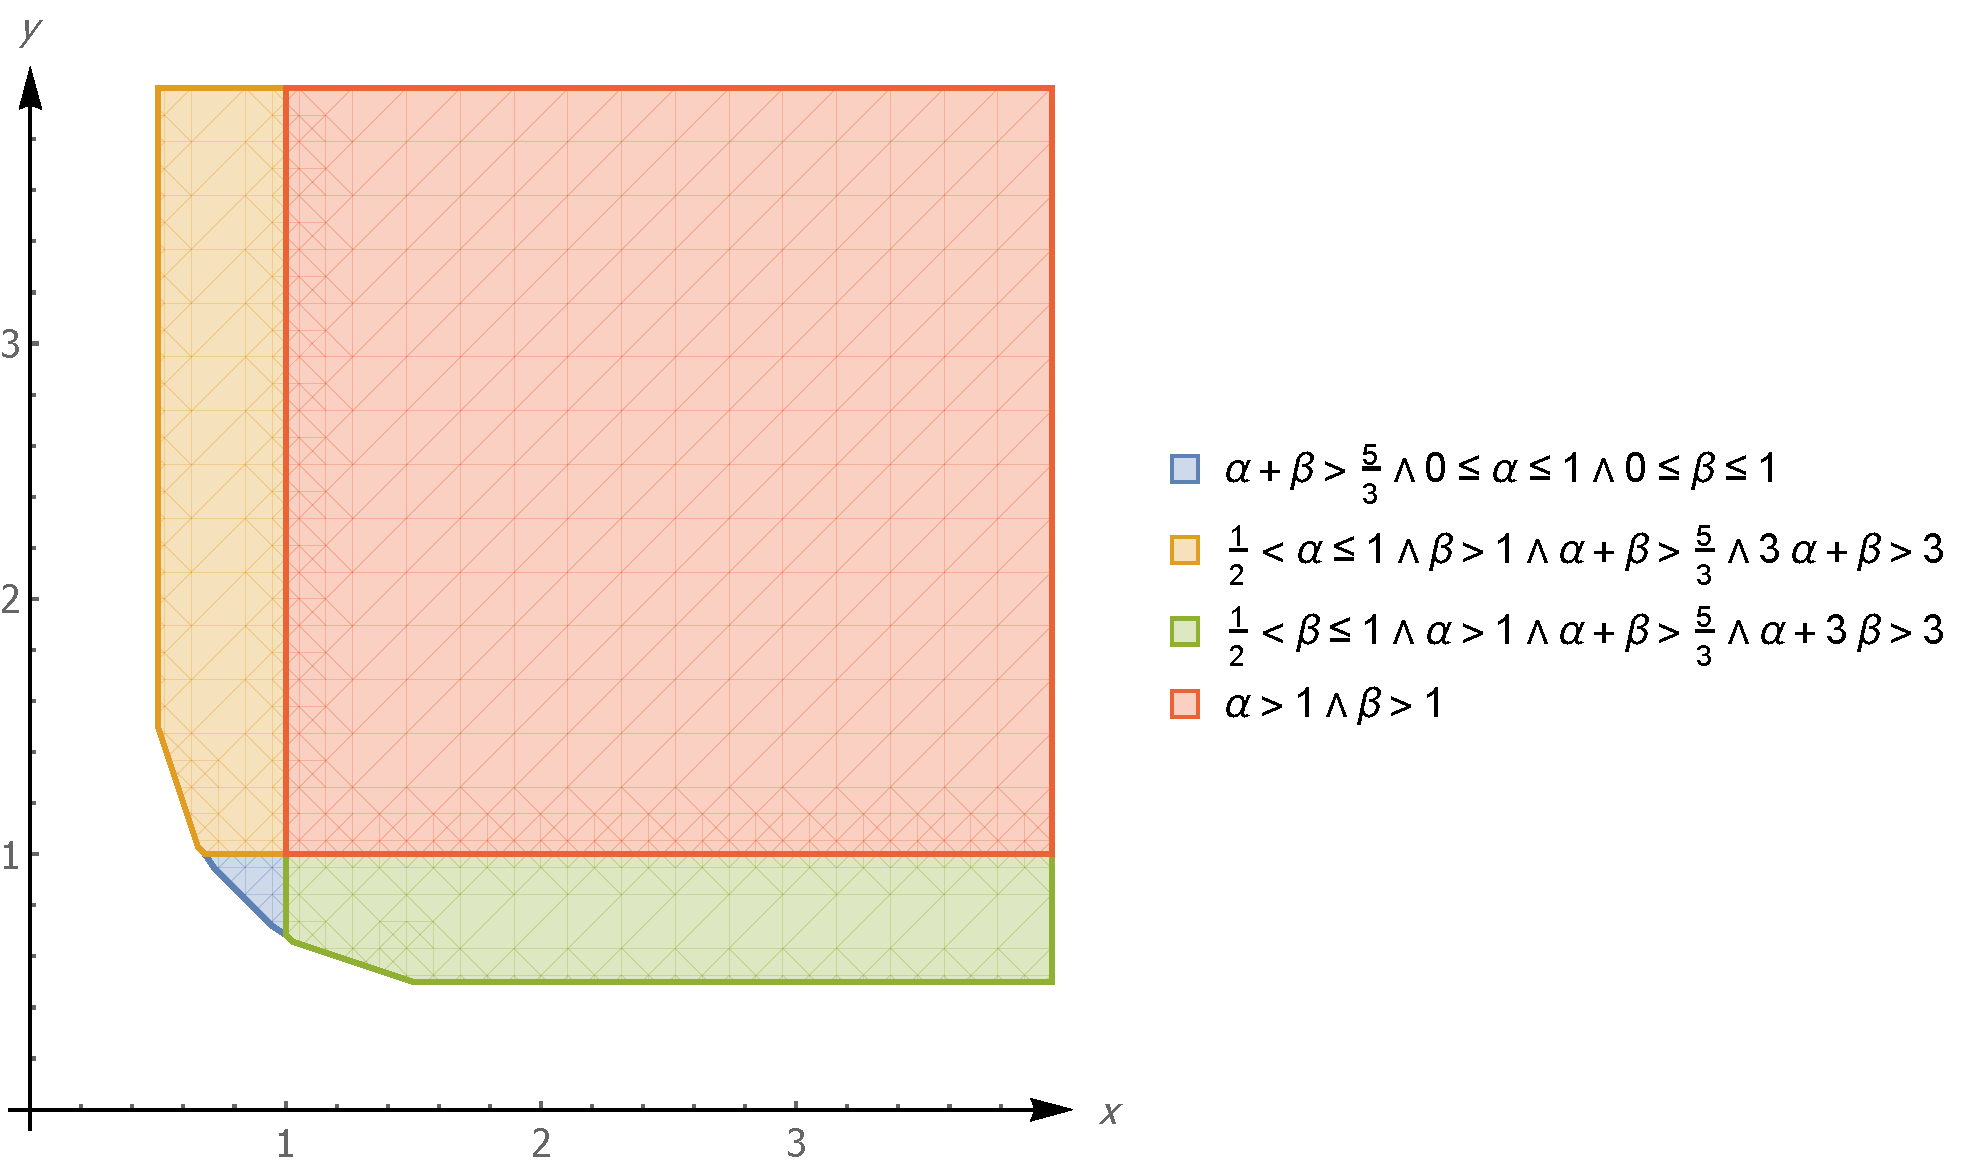
\includegraphics[width=14cm]{range.pdf}
    \centering
    \caption{Region that ensures the integral finite}
    \label{fig1}
    \end{figure}
    Combine all these four conditions we complete the proof.
 \end{proof}
To obtain Theorem \ref{thm-2}, we need the following important theorem in\cite[p.~60]{12}.
\begin{theorem}\label{thm-3}
    Let $u(t,x)$ be a mild solution of (\ref{kdv}). If there exists $t_1<t_2$ such that 
    \begin{equation}
        \mathrm{supp}u(\cdot, t_j)\subset (-\infty,c),\quad j=1,2
    \end{equation} 
    or 
    \begin{equation}
        \mathrm{supp}u(\cdot,t_j)\subset (c,\infty),\quad j=1,2
    \end{equation}
    for some $c\in \R$, then 
    $$
        u(x,t)\equiv 0,\quad -\infty <x,t<\infty.
    $$
\end{theorem}

\noindent {\itshape Proof of Theorem \ref{thm-2}}. Similar to the proof of Theorem \ref{thm-2}, we need to show $\|S(-t)T\|\neq 1$. It is equivalent to show that there does not exist nonzero function $f\in L^2(\R)$ such that $\| S(-t)Tf\|=\|f\|$. If not, then $\mathrm{supp}f\subset B$ and $\mathrm{supp}S(t)f\subset A$. But Theorem  \ref{thm-3} implies $f=0$, which makes a contradiction. \qed    
 
\section{Generalization}
\begin{definition}
    Let $S$ be a linear operator mapping the Hilbert space $(\mathcal{H}(R^n),\|\cdot\|)$ into itself and $E\subset \R^n$ be a measurable set. We call the operator $S$ antilocal with respect to $O$  if for any $f\in\mathcal{H}$ 
    $$
        \chi_Of=\chi_O Sf=0\Rightarrow f=0.
    $$
    If the above is true for any measurable set $|O|>0$, then we call the operator $S$ completely antilocal.   
\end{definition}
We can abstract and generalize the proof of Theorem \ref{thm-2} to the following theorem directly.
\begin{theorem}\label{thm-4}
    Let $(\mathcal{H}(\R^n),\|\cdot\|)$ be an infinite-dimensional complex Hilbert space. Let $A$ and $B$ be two measurable sets. Define $Ef=\chi_B f$ and $Ff=\chi_A f$. $S:\mathcal{H}\to \mathcal{H}$ is an invertible linear operator which satisfies $\|S^{-1}\| \|T\|<1$. If $S$ is antilocal with respect to some measurable set $O$ and $A,B\subset O $, then the inequalities (\ref{gen-1}) and (\ref{gen-2}) in Theorem \ref{thm-3} still holds.            
\end{theorem}
\begin{example}
    The Hilbert transform 
    $$
        Hf(x)\equiv \mathrm{p.v.}\frac{1}{\pi}\int_{\R}\frac{f(x-t)}{t}\d t
    $$
      is completely antilocal\cite[p.~485]{HavJor} and an isometry in $L^2(\R)$. Then we can use Theorem \ref{thm-4} to obtain the following: Let $A$ and $B$ be two measurable sets with finite measure, then there exists a constant $C=C(n,A,B)$  
    $$
        \int_{\R}|f|^2\d x\le C\left(\int_{A^c} |f|^2\d x+\int_{B^c}|Hf|^2\d x\right).
    $$
    
\end{example}
%\section*{Acknowledgements}

 %Wang was supported by the National Natural Science Foundation of China under grant No. 11701535.
\begin{thebibliography}{999}

{\scriptsize


 

\bibitem{L-Ponce14} F. Linares, G. Ponce, Introduction to nonlinear dispersive equations, 2nd edition. Springer, 2014.


 \bibitem{WWZ}  G. Wang, M. Wang, Y. Zhang, Observability and unique continuation inequalities for the Schr\"{o}dinger equation, J. Eur. Math. Soc.  21 (2019) 3513--3572.

\bibitem{12} B. Y. Zhang,   Unique continuation for the Korteweg-de Vries equation, SIAM J. Math. Anal. 32 (1992)  55--71.

  \bibitem{Zhang97} B. Y. Zhang,   Unique continuation for the nonlinear Schr\"odinger equation, Proc. Roy. Soc. Edinburgh Sect. A 127 (1997)  191--205.

  \bibitem{Amrein} W. O. Amerin, A. M. Berthier, On Support Properties of $L^p$-Functions and Their Fourier Transforms, J. Funct. Anal. 24 (1977) 258-267.
  }

  \bibitem{LW} Z. Li, M. Wang, Observability inequality at two time points for KdV equations, SIAM J. Math. Anal. to appear.

  \bibitem{HavJor} V. Havin, B. J\"{o}ricke, {\itshape The Uncertainty Principle in Harmonic Analysis}, Springer-Verlag, 1994.    
  \bibitem{Log} V. N. Logvinenko and J. F. Sereda, Equivariant norms in spaces of entire functions of exponential type, Teor. Funktsii Funktsional. Anal. i Prilozhen.,  20 (1974), pp. 102-111, 175 (in Russian).
  \bibitem{Korv} O.  Kovrijkine,Some  results  related  to  the  Logvinenko-Sereda  theorem,  Proc.  Amer.  Math.
  \bibitem{Rouss} J. Le Rousseau and I. Moyano, Null-controllability of the Kolmogorov equation in the whole phase space, J. Differential Equations, 260 (2016), pp. 3193--3233.
  \bibitem{WWZZ} G. Wang, M. Wang, C. Zhang, and Y. Zhang,Observable  set,  observability,  interpolation inequality  and  spectral  inequality  for  the  heat  equation  in $\mathbb{R}^{n}$, J. Math. Pures Appl., 126 (2019), pp. 144-194.
  \bibitem{Naza} F. L. Nazarov,Local estimates for exponential polynomials and their applications to inequalities  of  the  uncertainty  principle  type, Algebra i Analiz, 5 (1993), pp. 3--66 (in Russian); translation in St. Petersburg Math. J., 5 (1994), pp. 663--717.

\end{thebibliography}

\end{document}
